\subsection{Access control flows}
% NAME? "System flow example(s)

The access control flow of the proposed system can be broken down into three stages:
\begin{enumerate*}[label=(\roman*)]
    \item \textit{Authentication},
    \item \textit{Access Policy Evaluation} and
    \item \textit{Accessing protected resource}.
\end{enumerate*}
These stages can be identified in every use case of the system, although the flow in each stage is adapted to the given use case.

\subsubsection{Authentication}
In this stage, the user identifies and authenticates themselves to the \acrshort{aaserver}. This is the first stage of the access control flow and is only preceded by the user clicking a login button or approaching a door. The authentication is done via the FIDO2 protocol, but the flows during this stage are different during online login and when opening a door.

\paragraph{Authenticating online} During online authentication the user uses a browser or a native client application to communicate with the \acrshort{aaserver}. When the user clicks a login button, the client application redirects them to the login page, supplied by the \acrshort{aaserver}. The user agent/native client application needs to send a `Access request' message to the server, which contains these parameters: the \texttt{client\_id}, the callback URL, the requested scopes (and if the client is a native application, also the \acrshort{pkce} code challenge). The \texttt{client\_id} is immediately verified by the \acrshort{aaserver}. All variables are temporarily saved for use later in the process. 

The \acrshort{aaserver} provides a login form back to the requesting party. User enters their \acrshort{uid} into this form and chooses the authenticator they wish to use (physical key or smartphone). The filled form is then send back to the \acrshort{aaserver}. The server requests a login challenge for this \acrshort{uid} from the User directory. The User directory looks up the \acrshort{uid} in the user database and generates an Authentication assertion\footnotemark to be signed by the user's authenticator.
% 
\footnotetext{As defined by the WebAuthn specification:
% TODO reference "Web Authentication:An API for accessing Public Key Credentials Level 1"
\url{https://www.w3.org/TR/webauthn/\#dictdef-publickeycredentialrequestoptions}, accessed 08 April 2019}

If the user selected physical key as their authenticator, the Authentication assertion is then forwarded back to the user agent/native application that made the initial access request. If the user selected smartphone, the the Authentication assertion is forwarded to the Authentication front end. Once the signed assertion is received, the \acrshort{aaserver} forwards it to the User directory. User directory verifies that the signature was made by either of the public keys, associated with the \acrshort{uid}. The User directory then informs the \acrshort{aaserver} about the outcome of this verification.

In the last step of the Authentication stage, the \acrshort{aaserver} issues a signed and encrypted \acrshort{jwt} to the user agent/Authentication front end. This \acrshort{jwt} can be sent in the initial Access request and the remaining steps of the authentication stage are then skipped. The purpose of this is to avoid repeated authentication prompts to the user in a short time span (a couple of hours). Once the user authenticates using an authenticator on certain user agent, we do not need to prompt authentication on the same user agent again, until the validity of the \acrshort{jwt} has expired.

If a \acrshort{aaserver} receives a valid \acrshort{jwt} in the Access request, it does not carry out further authentication steps and proceeds directly to the Access policy evaluation stage. If the received \acrshort{jwt} is expired or otherwise invalid, the regular process described above applies.

Figure~\ref{fig:authentication-flow} illustrates this process in a sequence diagram. User authentication with a physical key is shown, when when logging in online to an internal or external application.
% TODO mention usecases here??!!
When authenticating with a smartphone and when using a \acrshort{pacs}, the flow would be slightly different.
% Please see Appendix
% TODO Add reference to full figures in appendix.

\paragraph{Authenticating to a \acrshort{pacs}} 
% As mentioned in 
% TODO point to a use case or something like that here
% the process of authentication and policy evaluation must be speedy.
The input form for the \acrshort{uid} is omitted and instead, the \acrshort{uid} is extracted directly from the authenticator.


\begin{sidewaysfigure}[ht]
    \centering
    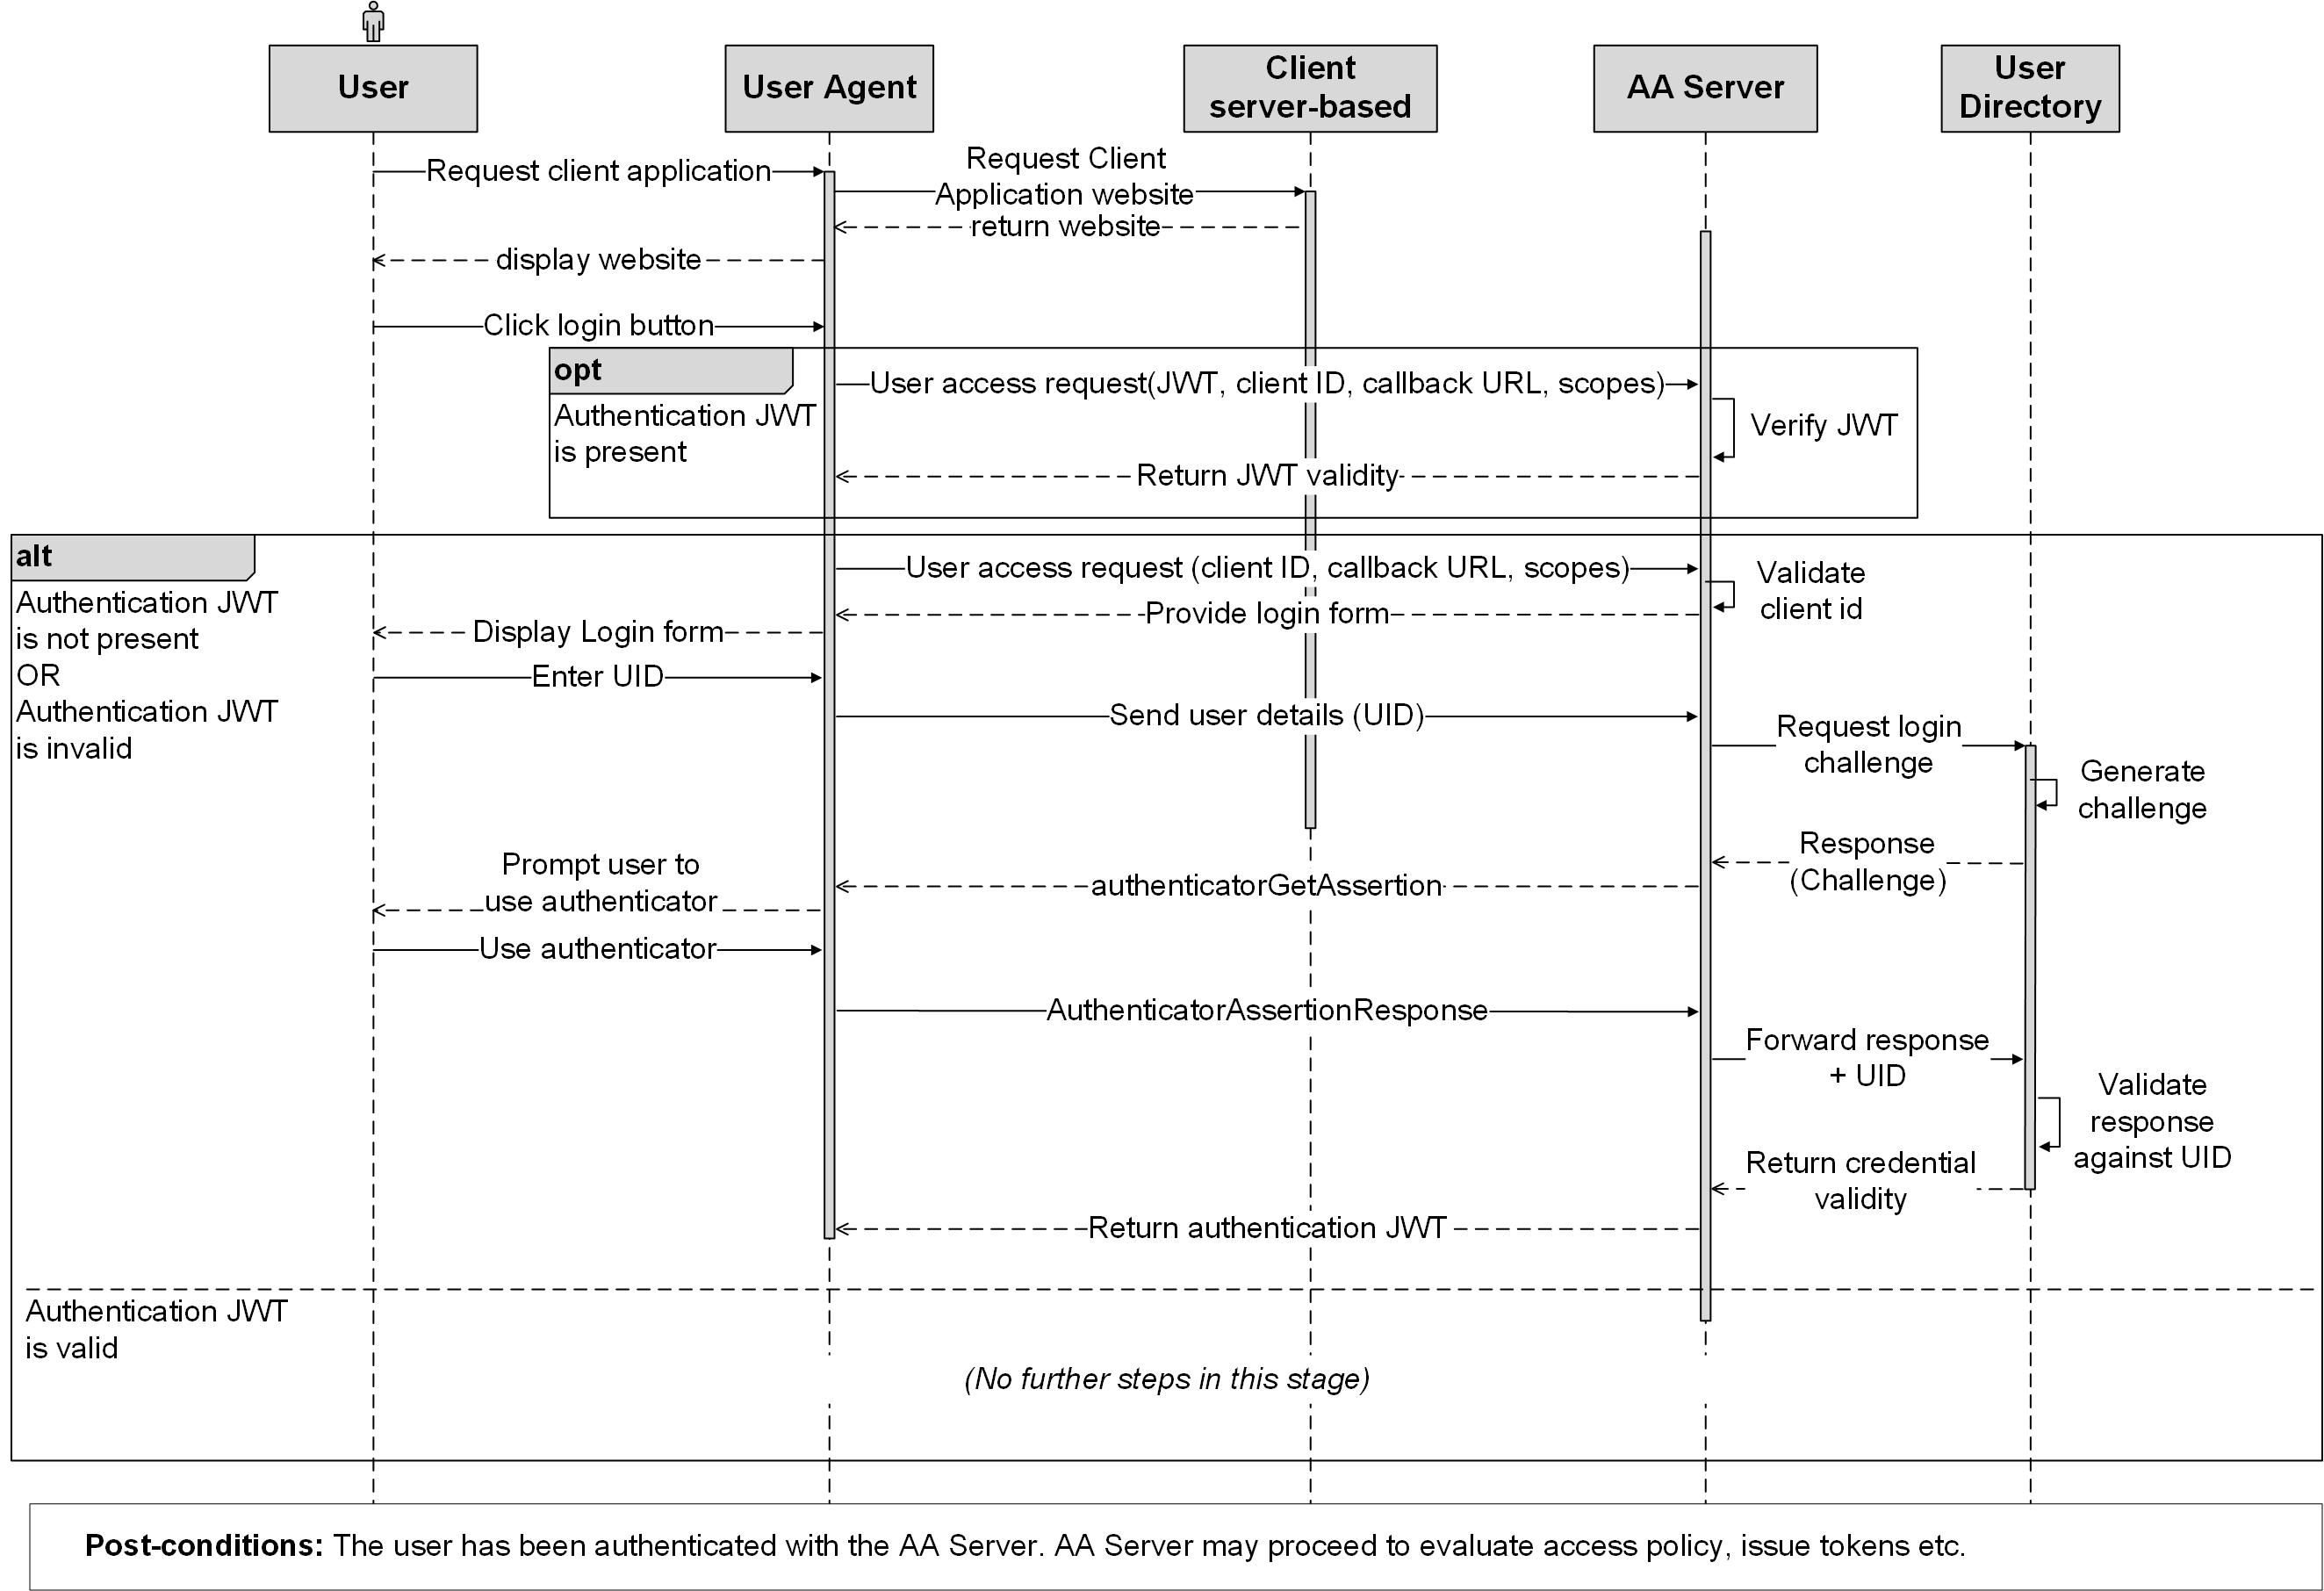
\includegraphics[width=\textwidth]{authentication-flow}
    \caption{Authentication flow during online access control with a server-based client, using a physical authenticator. If the authentication is not successful, the \acrshort{aaserver} informs the client and the user about the unsuccessful authentication and does not continue to the Access policy evaluation stage.}
    % TODO update figure with latest changes
    \label{fig:authentication-flow}
\end{sidewaysfigure}

\subsubsection{Access Policy Evaluation}
If the user supplied a valid authentication \acrshort{jwt} or if the user directory successfully verified the validity of the \texttt{AuthenticationAssertionResponse}, the \acrshort{aaserver} proceeds to the next stage -- Access policy evaluation. Involved in this stage are the \acrshort{aaserver}, the \acrshort{pdp} and, optionally the User Dictionary. The flow in this stage is the same when accessing an online application and the \acrshort{pacs}.

The flow begins by the \acrshort{aaserver} requesting access policy evaluation from the \acrshort{pdp} with a \texttt{CheckAccessPolicy} message. Included in this request are the \acrshort{uid}, the client identifier, the context of the request (

*tune of pink panther*
TO DO, TODO, TODO, TODO, TODOOOO....